\documentclass{article}

\usepackage[margin=1in]{geometry}
\usepackage{amsmath}
\usepackage{amssymb}
\usepackage{amsthm}
\usepackage{tikz}
\usepackage{listings}
\usepackage{hyperref}
\usepackage{xcolor}

\usetikzlibrary{arrows.meta,calc,3d}

\definecolor{codebg}{RGB}{245,245,245}
\definecolor{codekw}{RGB}{0,0,180}
\definecolor{codestr}{RGB}{160,32,32}
\definecolor{codecom}{RGB}{0,120,0}

\lstset{
  language=JavaScript,
  basicstyle=\ttfamily\footnotesize,
  backgroundcolor=\color{codebg},
  keywordstyle=\color{codekw}\bfseries,
  stringstyle=\color{codestr},
  commentstyle=\color{codecom}\itshape,
  breaklines=true,
  showstringspaces=false,
  numbers=left,
  numberstyle=\tiny\color{gray},
  frame=single,
  captionpos=b,
}

\title{Guide 04: Rotation Matrices and Euler Angles}
\author{web-3d-panel-navigation math curriculum}
\date{}

\begin{document}
\maketitle

\section{Why this matters}

Every zoom panel in this project is a flat rectangle floating in 3D space, and
the only thing that distinguishes one panel's orientation from another is its
\texttt{rotation} field --- a triple of Euler angles. The rotation is parsed
from a \texttt{data-rotation="x, y, z"} HTML attribute (in degrees) and
immediately converted to radians at parse time
(\texttt{src/zoom-plane-parser.ts:215}, where \lstinline|parseToThreeTuple| is
called with \lstinline|degreesToRadians| as the mapper). It is then stored on
\lstinline|ZoomPlaneConfig.rotation| as
\lstinline|[number, number, number]| in radians (see
\texttt{src/types.ts:24}). Three different files take that triple and reconstitute it as a
\lstinline|THREE.Euler(x, y, z, 'XYZ')| in order to: (1) place the four corners
of a panel in world space (\texttt{src/projection.ts:102--119}), (2) compute
the camera's perpendicular look-direction by rotating the standard basis
vectors $(0,0,1)$ and $(0,1,0)$ (\texttt{src/camera-controller.ts:59--69}),
and (3) compute the same normal again for the overview camera
(\texttt{src/overview-camera.ts:64--72}). To understand why the camera ends up
where it does --- and why panels with non-trivial rotations like
\texttt{"30, -15, 0"} land where they do --- you need rotation matrices and the
XYZ Euler convention. This guide builds that picture from scratch.

\section{Building intuition: 2D rotation}

Forget 3D for a moment. A 2D rotation takes a point on the plane and pivots
it around the origin by some angle $\theta$ (counter-clockwise is the universal
math convention). Look at what happens to the two basis vectors
$\hat{\mathbf{e}}_x = (1,0)$ and $\hat{\mathbf{e}}_y = (0,1)$.

\begin{center}
\begin{tikzpicture}[scale=2.5,>=Stealth]
  % axes
  \draw[->,gray] (-0.2,0) -- (1.4,0) node[right] {\small $x$};
  \draw[->,gray] (0,-0.2) -- (0,1.4) node[above] {\small $y$};

  % unit circle
  \draw[gray,dashed] (0,0) circle (1);

  % original basis
  \draw[->,thick,blue] (0,0) -- (1,0) node[below right] {$\hat{\mathbf{e}}_x$};
  \draw[->,thick,blue] (0,0) -- (0,1) node[above left] {$\hat{\mathbf{e}}_y$};

  % rotated basis (theta = 35 deg for picture)
  \draw[->,thick,red] (0,0) -- ({cos(35)},{sin(35)});
  \node[red] at ({cos(35)+0.18},{sin(35)-0.05}) {\small $R\hat{\mathbf{e}}_x$};
  \draw[->,thick,red] (0,0) -- ({-sin(35)},{cos(35)});
  \node[red] at ({-sin(35)-0.25},{cos(35)+0.05}) {\small $R\hat{\mathbf{e}}_y$};

  % angle arc
  \draw[->,thick] (0.45,0) arc (0:35:0.45);
  \node at (0.6,0.18) {\small $\theta$};
\end{tikzpicture}
\end{center}

\noindent The rotated $\hat{\mathbf{e}}_x$ slides counter-clockwise along the
unit circle, ending at angle $\theta$ from the positive $x$-axis. By the
definition of $\sin$ and $\cos$ on the unit circle (Guide 02), it lands at
$(\cos\theta, \sin\theta)$. The rotated $\hat{\mathbf{e}}_y$ is just
$\hat{\mathbf{e}}_x$ pivoted another $90^\circ$, so it lands at
$(\cos(\theta+90^\circ), \sin(\theta+90^\circ)) = (-\sin\theta, \cos\theta)$.

\section{The math}

\subsection{Deriving the 2D rotation matrix}

A linear map is fully determined by what it does to the basis vectors, and a
matrix is just a table whose columns are the images of the basis vectors. From
the picture:
\begin{align*}
R(\theta)\,\hat{\mathbf{e}}_x &= \begin{pmatrix}\cos\theta\\ \sin\theta\end{pmatrix}, &
R(\theta)\,\hat{\mathbf{e}}_y &= \begin{pmatrix}-\sin\theta\\ \cos\theta\end{pmatrix}.
\end{align*}
Stacking those two columns:
\begin{equation*}
R(\theta) = \begin{pmatrix}\cos\theta & -\sin\theta\\ \sin\theta & \cos\theta\end{pmatrix}.
\end{equation*}
Sanity check: $R(0) = I$ (identity, no rotation), $R(\pi/2)\begin{pmatrix}1\\0\end{pmatrix} = \begin{pmatrix}0\\1\end{pmatrix}$
(quarter-turn maps $+x$ to $+y$), and $\det R(\theta) = \cos^2\theta + \sin^2\theta = 1$
(rotations preserve area and orientation).

\subsection{The three 3D rotation matrices}

In 3D, a ``rotation'' needs an axis. Each of the three axis-aligned rotations
fixes one coordinate and acts as the 2D rotation of the previous section in the
plane spanned by the other two. The convention everyone uses (and Three.js
follows) is right-handed: point your right thumb along the positive axis and
your fingers curl in the direction of positive $\theta$.

\begin{equation*}
R_x(\theta) = \begin{pmatrix}
1 & 0 & 0\\
0 & \cos\theta & -\sin\theta\\
0 & \sin\theta & \cos\theta
\end{pmatrix},\quad
R_y(\theta) = \begin{pmatrix}
\cos\theta & 0 & \sin\theta\\
0 & 1 & 0\\
-\sin\theta & 0 & \cos\theta
\end{pmatrix},
\end{equation*}
\begin{equation*}
R_z(\theta) = \begin{pmatrix}
\cos\theta & -\sin\theta & 0\\
\sin\theta & \cos\theta & 0\\
0 & 0 & 1
\end{pmatrix}.
\end{equation*}

\noindent Note the sign pattern in $R_y$: because $y$ is the fixed axis, the
2D rotation lives in the $zx$-plane (in that order, to keep the right-handed
orientation), which flips the sign of one $\sin$ term compared to $R_x$ and
$R_z$. Mistaking that sign is the single most common bug in handwritten
rotation code; if you ever write your own, sanity-check by rotating
$(1,0,0)$ by $R_y(\pi/2)$ and confirming you get $(0,0,-1)$.

\subsection{Composition is matrix multiplication, and order matters}

Applying rotation $A$ and then rotation $B$ to a vector $\mathbf{v}$ gives
$B(A\mathbf{v}) = (BA)\mathbf{v}$. So composing rotations is multiplying
their matrices --- but with the catch that matrix multiplication is
\emph{not commutative}. Concretely, take $R_x(90^\circ)$ and $R_y(90^\circ)$:

\begin{equation*}
R_x(90^\circ) = \begin{pmatrix}1 & 0 & 0\\ 0 & 0 & -1\\ 0 & 1 & 0\end{pmatrix},\qquad
R_y(90^\circ) = \begin{pmatrix}0 & 0 & 1\\ 0 & 1 & 0\\ -1 & 0 & 0\end{pmatrix}.
\end{equation*}

Compute both products:
\begin{align*}
R_x(90^\circ)\,R_y(90^\circ) &= \begin{pmatrix}0 & 0 & 1\\ 1 & 0 & 0\\ 0 & 1 & 0\end{pmatrix},\\[4pt]
R_y(90^\circ)\,R_x(90^\circ) &= \begin{pmatrix}0 & 1 & 0\\ 0 & 0 & -1\\ -1 & 0 & 0\end{pmatrix}.
\end{align*}

\noindent These two matrices send the same starting vector to different
places. Try it on $\mathbf{v} = (1,0,0)$: the first product yields
$(0,1,0)$, the second yields $(0,0,-1)$. Rotating ``X then Y'' is not the
same as rotating ``Y then X''. This is exactly why an Euler triple is
meaningless without an order convention.

\subsection{Euler angles and Three.js's XYZ order}

An Euler angle decomposition writes a 3D rotation as a product of three
single-axis rotations. ``XYZ order'' could mean either of two things, so we
have to pin it down.

\textbf{Intrinsic} rotations are rotations about the body's \emph{current}
(already-rotated) axes, like a plane yawing then pitching about its own
nose-axis. \textbf{Extrinsic} rotations are about the fixed world axes. The
two are duals: an intrinsic XYZ sequence equals an extrinsic ZYX sequence,
and vice versa.

\textbf{Three.js's \lstinline|'XYZ'| convention.} The matrix that
\lstinline|THREE.Matrix4.makeRotationFromEuler| produces for an Euler with
\lstinline|order = 'XYZ'| is
\begin{equation*}
R = R_x(e_x)\,R_y(e_y)\,R_z(e_z),
\end{equation*}
when matrices act on column vectors from the left. Reading right-to-left as
the vector ``sees'' the operations: $R_z$ is applied first (about the world
$z$-axis), then $R_y$, then $R_x$. Equivalently, this is the
\emph{intrinsic XYZ} rotation: rotate about $X$ first, then about the new
$Y$, then about the new-new $Z$. (The two readings agree because they're
the same matrix; choose whichever picture is more comfortable.)

\textbf{What \lstinline|vector.applyEuler(new THREE.Euler(rx, ry, rz, 'XYZ'))| does.}
It replaces \lstinline|vector| with $R_x(r_x)\,R_y(r_y)\,R_z(r_z)\,\mathbf{v}$. In
this project that's exactly what's happening on every line listed in
Section~1: a fresh standard basis vector or a local-space corner gets the
plane's full rotation matrix applied to it.

\subsection{Gimbal lock}

Euler angles parameterize 3D rotations with three numbers, but the parameterization
is \emph{singular} at certain configurations: there are orientations where the
three angles fail to span all nearby orientations independently, so one degree of
freedom collapses. This is gimbal lock. For XYZ order, it happens when the middle
rotation $R_y(e_y) = R_y(\pm \pi/2)$ aligns the body's $X$ axis with the world's
$Z$ axis (or its negative). In that configuration $R_x$ and $R_z$ end up rotating
about the same axis, and the system can't distinguish $(e_x, e_z)$ from
$(e_x + \delta, e_z - \delta)$.

\begin{center}
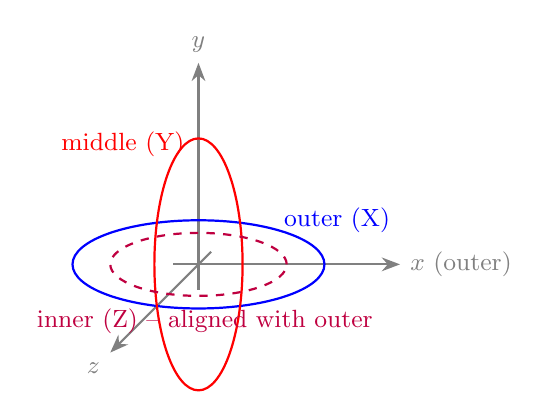
\begin{tikzpicture}[scale=1.6,>=Stealth]
  % world axes
  \draw[->,gray,thick] (-0.2,0) -- (1.6,0) node[right] {\small $x$ (outer)};
  \draw[->,gray,thick] (0,-0.2) -- (0,1.6) node[above] {\small $y$};
  \draw[->,gray,thick] (0.1,0.1) -- (-0.7,-0.7) node[below left] {\small $z$};

  % outer gimbal (around X) - drawn as ellipse
  \draw[blue,thick] (0,0) ellipse (1 and 0.35);
  \node[blue] at (1.1,0.35) {\small outer (X)};

  % middle gimbal rotated 90 deg around X so it now lies in the XZ plane
  \draw[red,thick,rotate around={90:(0,0)}] (0,0) ellipse (1 and 0.35);
  \node[red] at (-0.6,0.95) {\small middle (Y)};

  % inner gimbal: would normally rotate around Z, but Z now coincides with outer X axis
  \draw[purple,thick,dashed] (0,0) ellipse (0.7 and 0.25);
  \node[purple] at (0.05,-0.45) {\small inner (Z) -- aligned with outer};
\end{tikzpicture}
\end{center}

\noindent After a $90^\circ$ middle rotation, the inner $Z$ axis lies along
the outer $X$ axis: turning either gimbal produces the same motion, so
you've lost a degree of freedom. In code, gimbal lock shows up as
discontinuities --- two ``nearby'' orientations may have wildly different
Euler triples. Quaternions (Guide 05) eliminate this entirely.

\section{In this codebase}

The project's \lstinline|rotation| field is parsed at one site and consumed
at three. Below are the verbatim snippets, each with the math written out.

\subsection{Parsing: degrees in, radians stored}

From \texttt{src/zoom-plane-parser.ts:215} (and the supporting
\lstinline|parseToThreeTuple| above it):

\begin{lstlisting}[caption={zoom-plane-parser.ts (excerpt)}]
function degreesToRadians(degrees: number): number {
  return (degrees * Math.PI) / 180;
}

// ...

return {
  // ...
  rotation: parseToThreeTuple(rotationStr, id, 'rotation', degreesToRadians),
  // ...
};
\end{lstlisting}

\noindent An attribute \texttt{data-rotation="0, 30, 0"} becomes the triple
$(0,\ \pi/6,\ 0)$ stored on \lstinline|config.rotation|. From here on,
the package treats the three numbers as the Euler triple
$(e_x, e_y, e_z)$ in radians, in XYZ order.

\subsection{Placing corners in world space}

From \texttt{src/projection.ts:84--120}:

\begin{lstlisting}[caption={projection.ts: getPlaneWorldCorners (excerpt)}]
const localCorners = [
  new THREE.Vector3(-halfWidth,  halfHeight, 0),  // top-left
  new THREE.Vector3( halfWidth,  halfHeight, 0),  // top-right
  new THREE.Vector3( halfWidth, -halfHeight, 0),  // bottom-right
  new THREE.Vector3(-halfWidth, -halfHeight, 0),  // bottom-left
];

const euler = new THREE.Euler(
  config.rotation[0],
  config.rotation[1],
  config.rotation[2]
);
// ...
return localCorners.map(corner => {
  const worldCorner = corner.clone();
  worldCorner.applyEuler(euler);
  worldCorner.add(position);
  return worldCorner;
});
\end{lstlisting}

\noindent A panel is born flat in the $xy$-plane, $z=0$, facing
$+\hat{\mathbf{z}}$. Each corner $\mathbf{c}_\text{local}$ is mapped to
world space by
\begin{equation*}
\mathbf{c}_\text{world} = R_x(e_x)\,R_y(e_y)\,R_z(e_z)\,\mathbf{c}_\text{local} + \mathbf{p},
\end{equation*}
where $\mathbf{p} = $ \lstinline|config.position|. Note that the
\lstinline|new THREE.Euler(...)| call here omits the order argument; the
default order in Three.js is \lstinline|'XYZ'|, so this is the same as the
explicit \lstinline|'XYZ'| used elsewhere.

\subsection{Rotating the standard basis to get a frame}

From \texttt{src/camera-controller.ts:59--69}:

\begin{lstlisting}[caption={camera-controller.ts: calculatePerpendicularState (excerpt)}]
const euler = new THREE.Euler(
  plane.rotation[0], plane.rotation[1], plane.rotation[2]
);

// Plane's normal vector (perpendicular, pointing toward viewer)
const normal = new THREE.Vector3(0, 0, 1);
normal.applyEuler(euler);
normal.normalize();

// Plane's local "up" vector
const planeUp = new THREE.Vector3(0, 1, 0);
planeUp.applyEuler(euler);
planeUp.normalize();
\end{lstlisting}

\noindent This is the project's most important pattern. A panel's geometric
identity --- where it faces, which way is up on it --- is whatever the
identity panel's basis becomes after applying the rotation. Concretely:
\begin{align*}
\mathbf{n} &= R\,(0,0,1)^\top &&\text{(panel normal: where it faces)}\\
\mathbf{u} &= R\,(0,1,0)^\top &&\text{(panel up)}
\end{align*}
where $R = R_x(e_x)\,R_y(e_y)\,R_z(e_z)$. The camera then sits at
$\mathbf{p} + d\,\mathbf{n}$ and looks back at $\mathbf{p}$ with $\mathbf{u}$ as
its world ``up''. Guide 06 will dignify $(\mathbf{r}, \mathbf{u}, \mathbf{n})$
with the name \emph{local frame}; for now it is just the basis pattern.

\subsection{Same pattern, overview camera}

From \texttt{src/overview-camera.ts:64--72}, the focal-element overview reuses
the trick on the center plane:

\begin{lstlisting}[caption={overview-camera.ts: calculateFocalElementMode (excerpt)}]
const normal = new THREE.Vector3(0, 0, 1);
const euler = new THREE.Euler(
  centerPlane.rotation[0],
  centerPlane.rotation[1],
  centerPlane.rotation[2]
);
normal.applyEuler(euler);
normal.normalize();
\end{lstlisting}

\noindent Rotate $(0,0,1)$ by the panel's Euler triple, get a unit-length
direction in world space pointing perpendicular to the panel. The overview
camera will be placed along that direction at whatever distance fits all
panels in frame.

\section{Worked examples}

\subsection*{Example 1: A pure yaw}

\textbf{Setup.} A panel with \lstinline|data-rotation="0, 30, 0"|. After
parsing, $(e_x, e_y, e_z) = (0,\ \pi/6,\ 0)$ radians.

\textbf{Question.} What is the panel's normal in world space?

\textbf{Solution.} With $e_x = e_z = 0$, the matrix is just
$R = R_y(\pi/6)$. The normal is
\begin{equation*}
\mathbf{n} = R_y(\pi/6) \begin{pmatrix}0\\0\\1\end{pmatrix} = \begin{pmatrix}\cos(\pi/6) & 0 & \sin(\pi/6)\\ 0 & 1 & 0\\ -\sin(\pi/6) & 0 & \cos(\pi/6)\end{pmatrix}\begin{pmatrix}0\\0\\1\end{pmatrix} = \begin{pmatrix}\sin(\pi/6)\\ 0\\ \cos(\pi/6)\end{pmatrix} = \begin{pmatrix}1/2\\ 0\\ \sqrt{3}/2\end{pmatrix}.
\end{equation*}
So the panel still faces ``mostly toward $+z$'' but is yawed
$30^\circ$ toward $+x$. The camera will be placed at
$\mathbf{p} + d\,(1/2,\ 0,\ \sqrt{3}/2)$.

\subsection*{Example 2: Where do the corners go?}

\textbf{Setup.} Same panel as Example 1, with width $1600$ and height
$900$ (numbers chosen to match the ``half-corners'' of $\pm 800,\ \pm 450$
that the project routinely deals with), at position $\mathbf{p} = \mathbf{0}$
for simplicity.

\textbf{Question.} Where does the corner $\mathbf{c}_\text{local} = (800,\ 450,\ 0)$ land?

\textbf{Solution.} The local-space corner is in the panel's plane (third
component zero), so $R_y$ acts on its $x$ and $z$ components:
\begin{equation*}
R_y(\pi/6)\begin{pmatrix}800\\ 450\\ 0\end{pmatrix} = \begin{pmatrix}800\cos(\pi/6) + 0\\ 450\\ -800\sin(\pi/6) + 0\end{pmatrix} = \begin{pmatrix}800\cdot\tfrac{\sqrt{3}}{2}\\ 450\\ -800\cdot\tfrac12\end{pmatrix} \approx \begin{pmatrix}692.8\\ 450\\ -400\end{pmatrix}.
\end{equation*}
The other corners follow the same recipe: $y$ unchanged, $(x, z)$ rotated by
$30^\circ$ in the $xz$-plane. Notice that the corner moved
\emph{into} negative $z$ (away from the camera) on its right side, exactly
what you'd expect from a panel turned to face slightly to its right.

\subsection*{Example 3: Order really matters}

\textbf{Setup.} A panel with \lstinline|data-rotation="90, 90, 0"|. After
parsing, $(e_x, e_y, e_z) = (\pi/2,\ \pi/2,\ 0)$.

\textbf{Question.} What's the normal? And what would it be if Three.js used
ZYX order instead?

\textbf{Solution.} XYZ order: $\mathbf{n} = R_x(\pi/2)\,R_y(\pi/2)\,(0,0,1)^\top$.
First $R_y(\pi/2)\,(0,0,1)^\top = (1, 0, 0)^\top$ (pure-yaw $90^\circ$ swings the
$+z$ vector to $+x$). Then $R_x(\pi/2)\,(1,0,0)^\top = (1,0,0)^\top$ ($R_x$
fixes the $x$-axis). So $\mathbf{n} = (1, 0, 0)$.

ZYX order: $\mathbf{n} = R_z(0)\,R_y(\pi/2)\,R_x(\pi/2)\,(0,0,1)^\top$.
First $R_x(\pi/2)\,(0,0,1)^\top = (0, -1, 0)^\top$ (pitch swings $+z$ to $-y$).
Then $R_y(\pi/2)\,(0,-1,0)^\top = (0, -1, 0)^\top$ ($R_y$ fixes the $y$-axis).
$R_z(0)$ does nothing. So $\mathbf{n} = (0, -1, 0)$.

The same triple of numbers gives a panel facing $+x$ under XYZ but a panel
facing $-y$ under ZYX. Order is not a detail; it's part of the data.

\section{Exercises}

\begin{enumerate}
\item Compute $R_y(45^\circ)$ applied to the vector $(1,0,0)$. Then to $(0,0,1)$. Sketch both.

\item A panel has \lstinline|data-rotation="0, 0, 90"|. What is its normal?
Its up vector? Why does this rotation feel like it does ``nothing visible''
when viewed from $+z$, and what does it actually change?

\item Verify by direct multiplication that
$R_x(90^\circ)R_y(90^\circ) \neq R_y(90^\circ)R_x(90^\circ)$ on the test
vector $(1,1,0)$. Show what each side gives.

\item (Conceptual.) Why does Euler-order matter for storage and parsing
but not, say, for the dot product of two world-space normals?

\item (Project-applied.) If you swapped Three.js's order from
\lstinline|'XYZ'| to \lstinline|'ZYX'| everywhere in the project, what
would \lstinline|data-rotation="0, 30, 0"| do differently? What about
\lstinline|data-rotation="30, 0, 0"|?

\item (Project-applied.) The function
\lstinline|getPlaneWorldCorners| in
\texttt{src/projection.ts} constructs the Euler without an order argument:
\lstinline|new THREE.Euler(rx, ry, rz)|. Will the corners come out the same
as if it had passed \lstinline|'XYZ'| explicitly? Why?

\item Show that for any rotation matrix $R \in SO(3)$ and any unit vector
$\mathbf{v}$, the result $R\mathbf{v}$ is also a unit vector. (Hint:
$|R\mathbf{v}|^2 = (R\mathbf{v})^\top(R\mathbf{v}) = \mathbf{v}^\top R^\top R \mathbf{v}$,
and $R^\top R = I$.) Why does this make the
\lstinline|.normalize()| call in \lstinline|calculatePerpendicularState| a
defensive belt-and-suspenders move rather than a strict necessity?
\end{enumerate}

\textbf{Extension challenges.}
\begin{enumerate}\setcounter{enumi}{7}
\item Find a non-trivial Euler triple in XYZ order whose middle rotation
$e_y$ is exactly $\pi/2$. Show explicitly that varying $e_x$ by $\delta$ and
$e_z$ by $-\delta$ gives the \emph{same} final rotation matrix, illustrating
gimbal lock.

\item Three.js stores rotations internally as quaternions, but the project
exposes them as Euler triples on \lstinline|ZoomPlaneConfig|. Read
\texttt{src/zoom-plane-parser.ts:489}. After tile composition, the code calls
\lstinline|new THREE.Euler().setFromQuaternion(quaternion, 'XYZ')|. Why is
that final conversion necessary, and what would go wrong if the order
argument disagreed with the order used elsewhere in the package?
\end{enumerate}

\section{Where to next}

The two pain points of this guide --- gimbal lock, and the awkwardness of
multiplying $R_x$, $R_y$, $R_z$ to compose rotations during tiling --- both
disappear with quaternions. Guide 05 introduces them as a four-number
parameterization that has no singularities and composes cleanly via a
single multiplication. Once you've seen quaternions you'll understand why
the tiling code in
\lstinline|resolveTiledPlane| (\texttt{src/zoom-plane-parser.ts:406--496})
does its rotation arithmetic in quaternion-land and only converts back to
Euler at the very end via
\lstinline|new THREE.Euler().setFromQuaternion(quaternion, 'XYZ')|. After
quaternions, Guide 06 names the basis-vector triple from
Section~4.3 (\emph{the local frame}) and ties it to camera placement
in earnest.

\appendix
\section{Appendix: Solutions}

\textbf{Exercise 1.}
\begin{align*}
R_y(45^\circ)\begin{pmatrix}1\\0\\0\end{pmatrix} &= \begin{pmatrix}\cos 45^\circ\\ 0\\ -\sin 45^\circ\end{pmatrix} = \begin{pmatrix}\sqrt{2}/2\\ 0\\ -\sqrt{2}/2\end{pmatrix},\\
R_y(45^\circ)\begin{pmatrix}0\\0\\1\end{pmatrix} &= \begin{pmatrix}\sin 45^\circ\\ 0\\ \cos 45^\circ\end{pmatrix} = \begin{pmatrix}\sqrt{2}/2\\ 0\\ \sqrt{2}/2\end{pmatrix}.
\end{align*}
Both vectors stay in the $xz$-plane and rotate $45^\circ$ within it.

\textbf{Exercise 2.} With $(e_x, e_y, e_z) = (0, 0, \pi/2)$, the rotation is
$R_z(\pi/2)$. The normal: $R_z(\pi/2)\,(0,0,1)^\top = (0,0,1)^\top$ (the
$z$-axis is fixed by $R_z$). So the panel still faces $+z$. The up vector:
$R_z(\pi/2)\,(0,1,0)^\top = (-1, 0, 0)^\top$ --- the panel's local up now
points in the world $-x$ direction. From a $+z$ vantage the panel looks
identical, but it's been \emph{rolled} $90^\circ$. The camera's
\lstinline|up| vector reflects this, so on screen the panel's content
appears rotated $90^\circ$.

\textbf{Exercise 3.} Using the products from Section~3.3:
\begin{align*}
R_x(90^\circ)R_y(90^\circ)\begin{pmatrix}1\\1\\0\end{pmatrix} &= \begin{pmatrix}0&0&1\\1&0&0\\0&1&0\end{pmatrix}\begin{pmatrix}1\\1\\0\end{pmatrix} = \begin{pmatrix}0\\1\\1\end{pmatrix},\\
R_y(90^\circ)R_x(90^\circ)\begin{pmatrix}1\\1\\0\end{pmatrix} &= \begin{pmatrix}0&1&0\\0&0&-1\\-1&0&0\end{pmatrix}\begin{pmatrix}1\\1\\0\end{pmatrix} = \begin{pmatrix}1\\0\\-1\end{pmatrix}.
\end{align*}
Different vectors; non-commutative.

\textbf{Exercise 4.} The order matters because the same numerical triple
$(e_x, e_y, e_z)$ corresponds to \emph{different} rotation matrices under
different orderings (Example 3 demonstrated this). Storage and parsing
need to fix a convention so that everyone reading the data agrees on the
rotation it encodes. Once the rotation has been turned into world-space
vectors, those vectors have no remaining order-dependence; geometric
operations on them (dot product, cross product, etc.) are convention-free.

\textbf{Exercise 5.} Under XYZ, \lstinline|"0, 30, 0"| gave normal
$(\sin 30^\circ, 0, \cos 30^\circ)$ (Example 1). Under ZYX, the same triple
yields $R_z(0)\,R_y(\pi/6)\,R_x(0)\,(0,0,1)^\top = R_y(\pi/6)\,(0,0,1)^\top$,
which gives the \emph{same} normal. Single-axis rotations (only one
non-zero component) commute trivially across orderings, so
\lstinline|"30, 0, 0"| also behaves identically. Order-swap effects only
become visible when at least two of the three Euler angles are non-zero.

\textbf{Exercise 6.} The default order for \lstinline|new THREE.Euler(rx, ry, rz)|
in Three.js is \lstinline|'XYZ'|, so it is identical to the explicit
\lstinline|'XYZ'| used in \texttt{zoom-plane-parser.ts:422} and elsewhere.
The corners come out the same. (It's still better practice to be explicit;
the current code relies on a Three.js default never changing.)

\textbf{Exercise 7.} Rotation matrices are orthogonal: $R^\top R = I$. Then
$|R\mathbf{v}|^2 = \mathbf{v}^\top R^\top R \mathbf{v} = \mathbf{v}^\top \mathbf{v} = |\mathbf{v}|^2$,
so rotations preserve length. Since $(0,0,1)$ and $(0,1,0)$ start with
length 1, \lstinline|.applyEuler| leaves them with length 1, and
\lstinline|.normalize()| changes nothing in exact arithmetic. In floating
point it can correct tiny drift but is otherwise redundant.

\textbf{Exercise 8.} Take $(e_x, e_y, e_z) = (\theta, \pi/2, \phi)$ for any
$\theta, \phi$. The intuition: with $e_y = \pi/2$, $R_y$ swings the body's
$X$ axis onto the world $-Z$ axis, so the subsequent $R_x$ rotation, which
acts about the body's $X$-axis, ends up rotating about world-$-Z$.
Meanwhile $R_z$, applied first, rotates about world $Z$. Both end up
generating rotations about the same world axis, just with opposite signs.

To verify directly, multiply $R = R_x(e_x)\,R_y(\pi/2)\,R_z(e_z)$. With
$c_z = \cos e_z$, $s_z = \sin e_z$, $c_x = \cos e_x$, $s_x = \sin e_x$:
\[
  R_y(\pi/2)\,R_z(e_z) = \begin{pmatrix} 0 & 0 & 1 \\ 0 & 1 & 0 \\ -1 & 0 & 0 \end{pmatrix}
                          \begin{pmatrix} c_z & -s_z & 0 \\ s_z & c_z & 0 \\ 0 & 0 & 1 \end{pmatrix}
                        = \begin{pmatrix} 0 & 0 & 1 \\ s_z & c_z & 0 \\ -c_z & s_z & 0 \end{pmatrix}.
\]
Left-multiplying by $R_x(e_x) = \begin{pmatrix} 1 & 0 & 0 \\ 0 & c_x & -s_x \\ 0 & s_x & c_x \end{pmatrix}$
and using the angle-sum identities $c_x c_z - s_x s_z = \cos(e_x + e_z)$ and
$c_x s_z + s_x c_z = \sin(e_x + e_z)$:
\[
  R = \begin{pmatrix} 0 & 0 & 1 \\
                      \sin(e_x + e_z) & \cos(e_x + e_z) & 0 \\
                      -\cos(e_x + e_z) & \sin(e_x + e_z) & 0 \end{pmatrix}.
\]
$R$ depends on $e_x$ and $e_z$ \emph{only through the sum} $e_x + e_z$.
Shifting $e_x$ by $\delta$ and $e_z$ by $-\delta$ keeps $e_x + e_z$
unchanged, so $R$ is unchanged: two parameters control one degree of freedom
--- gimbal lock. (You can verify this in the browser console with
\lstinline|new THREE.Euler(0.1, Math.PI/2, 0.0).toMatrix4()| versus
\lstinline|new THREE.Euler(0.2, Math.PI/2, -0.1).toMatrix4()|; both produce
the same matrix up to floating-point noise.)

\textbf{Exercise 9.} \lstinline|setFromQuaternion(quaternion, 'XYZ')| asks
``what XYZ-order Euler triple represents the same rotation as this
quaternion?'' --- a one-to-one decomposition (away from gimbal lock).
The conversion is necessary because the rest of the package (parser
output, projection, camera controllers) consumes Euler triples; if the
tiling code returned a quaternion, every downstream consumer would have to
change. Passing a different order argument here than is used in
\texttt{projection.ts} or \texttt{camera-controller.ts} would mean the same
panel has two different ``valid'' Euler triples that produce different
orientations when later reconstructed --- so corners and camera would
disagree on where the panel points. Order-consistency across the package
is load-bearing.

\end{document}
